\documentclass[11pt]{amsart}
\usepackage{amsmath,amssymb,amsthm}
\usepackage{graphicx}
\usepackage{booktabs}
\usepackage{hyperref}
\usepackage[margin=1in]{geometry}
% allow a little inter-paragraph stretch so page breaks are not underfull
\raggedbottom
\graphicspath{{./}}

\newtheorem{theorem}{Theorem}
\newtheorem{corollary}{Corollary}
\newtheorem{conjecture}{Conjecture}
\newtheorem{remark}{Remark}
\theoremstyle{definition}
\newtheorem{definition}{Definition}

\newcommand{\Lsym}[2]{\left(\tfrac{#1}{#2}\right)}
\newcommand{\Art}{\mathrm{Art}}
\newcommand{\E}{\mathbb{E}}

\begin{document}

\title[Correlations between primitive root statuses of consecutive primes]{Correlations between primitive root statuses\\ of consecutive primes}

\author{Josh Bald}
\thanks{\textbf{Corresponding author.} Josh Bald, Independent Researcher.
	Email: \texttt{jpbald93@gmail.com}. ORCID: \texttt{0009-0002-1317-6489}.}

\date{September 10, 2026}

\subjclass[2020]{Primary 11A07; Secondary 11N05, 11N13, 11Y16, 11Y60}
\keywords{Artin's primitive root conjecture, primitive roots, consecutive primes,
	Lemke Oliver--Soundararajan bias, quadratic residues, Legendre symbol,
	full reptend primes, computational number theory}

\begin{abstract}
	Call a prime $p$ an \emph{Artin prime for base $10$} if $10$ is a primitive root
	modulo $p$. We investigate the dependence between the Artin
	statuses of \emph{consecutive} primes. Computing Artin status for all
	$50{,}847{,}531$ primes $7 \le p \le 10^9$, we find that consecutive primes are
	measurably \emph{anticorrelated}: $P(\Art_{n+1} \mid \Art_n) = 0.36514$
	versus $P(\Art_{n+1} \mid \lnot\Art_n) = 0.37928$, a deficit
	$\delta = -0.01414$ (Pearson statistic $10{,}167$ on one degree of freedom;
	signed square root $-100.8$ under a nominal independent-status reference model;
	over $50{,}847{,}530$ consecutive pairs).
	The dependence has striking gap structure. We prove an elementary exclusion law:
	if $p, p + g > 5$ are both prime with
	$g \equiv 20 \pmod{40}$, then $10$ is a quadratic residue modulo exactly one of
	them, so they can never both be Artin primes for base $10$; empirically, among
	$2{,}195{,}882$ consecutive pairs with gap $20$ or $60$ there is indeed not a
	single doubly-Artin pair; an independent recomputation extends this to
	$194{,}296{,}748$ such pairs below $10^{11}$, again with none.
	Conversely, gaps $g \equiv 0 \pmod{40}$ force equal
	quadratic-residue status and exhibit strong positive dependence
	($P(\Art_{n+1} \mid \Art_n) = 0.899$ at $g = 40$). Conditioning on the joint
	residues of $(p_n, p_{n+1})$ modulo $120$ or $840$ substantially reduces a
	selected-cell signed residual association; the remaining association is small in
	that metric but is not established to vanish. These results are consistent with
	a substantial role for arithmetic residue structure in the observed
	anticorrelation; they do not constitute a complete decomposition or an
	independent quantitative verification of the Hardy--Littlewood explanation.
	As an intermediate link we report the (apparently unreported) anticorrelation
	$r\bigl(\omega(p_n - 1), \omega(p_{n+1} - 1)\bigr) = -0.041$.
	At four decade-spaced cutoffs $x = 10^8, 10^9, 10^{10}, 10^{11}$ the deficit
	grows in magnitude with decreasing increments,
	$\delta = -0.01336, -0.01414, -0.01472, -0.01500$, and no turnover is
	observed; we draw no asymptotic conclusion from this, and in particular these
	finite-range values do not distinguish eventual decay to zero from
	persistence of a nonzero correlation.
	We formulate open questions and discuss extensions to general bases.
\end{abstract}

\maketitle

\section{Introduction}
\label{sec:intro}

Two classical themes in the theory of primes intersect in this paper.

The first is Artin's primitive root conjecture, communicated to Hasse in 1927
(see~\cite{Artin1965} and the historical account in~\cite{Moree2012}): for any integer
$a \notin \{-1, 0, 1\}$ that is not a perfect square, the set of primes $p$ for
which $a$ is a primitive root modulo $p$ has positive density relative to
the primes; for base
$a = 10$ this density is Artin's constant
$C = \prod_q \bigl(1 - \tfrac{1}{q(q-1)}\bigr) \approx 0.3739558$.
Hooley~\cite{Hooley1967} proved the conjecture under the Generalized Riemann
Hypothesis. Unconditionally, Gupta and Murty~\cite{GuptaMurty1984} and
Heath-Brown~\cite{HeathBrown1986} showed that the conjecture can fail for at
most two prime values of~$a$, though without an asymptotic for the counting
function; in the averaged direction Klurman, Shparlinski and
Ter\"av\"ainen~\cite{KlurmanShparlinskiTeravainen2025} recently established the
predicted asymptotic for almost all $1 \le a \le \exp((\log\log x)^2)$,
substantially improving the range of Stephens~(1969). Moree's
survey~\cite{Moree2012} gives a comprehensive account.
For $a = 10$ the property has a pleasant classical meaning: $10$ is a primitive
root mod $p$ precisely when the decimal expansion of $1/p$ has maximal period
$p - 1$ (the \emph{full reptend} or \emph{long} primes; see
\cite[pp.~166--171]{ConwayGuy1996}).

The second theme is the surprising dependence between \emph{consecutive}
primes quantitatively investigated and conjecturally explained by Lemke Oliver
and Soundararajan~\cite{LOS2016} (earlier numerical observations of such
biases are due to Knapowski--Tur\'an, Ko, and Ash--Beltis--Gross--Sinnott, as
\cite{LOS2016} itself discusses): for a
modulus $q$, a prime in a given reduced residue class mod $q$ is followed by a
prime in the \emph{same} class markedly less often than equidistribution would
predict. The phenomenon, which they explain conjecturally via the
Hardy--Littlewood prime $k$-tuple conjectures~\cite{HardyLittlewood1923}, decays
slowly and is prominent at the scales accessible to computation.

This paper asks a correlational question: \emph{are the Artin statuses of
consecutive primes correlated?} The adjacent question of when two primes at a
fixed even shift can \emph{both} be Artin primes was taken up by Tinkov\'a,
Waxman and Zindulka~\cite{TinkovaWaxmanZindulka2023}, whose Theorem~1.1
identifies shift--base pairs admitting no such pair; the exclusion law of
Theorem~\ref{thm:exclusion} below is the base-$10$ instance of that
phenomenon and we claim no priority for it. The correlation measured here,
over consecutive primes rather than a fixed shift, appears not to have been
studied. Since the
Artin property of $p$ is governed by the arithmetic of $p - 1$ (which primes
$q$ divide it), and since the residues of consecutive primes modulo small $q$
are correlated by~\cite{LOS2016}, one expects \emph{some} induced dependence
between $\mathbf{1}[10 \text{ is a primitive root mod } p_n]$ and
$\mathbf{1}[10 \text{ is a primitive root mod } p_{n+1}]$. What is not obvious
is its sign, its size, its structure as a function of the gap
$g = p_{n+1} - p_n$, or the extent to which it is connected to known
arithmetic structure. We answer these questions computationally for all primes up to
$10^9$ and isolate one component that is not merely statistical but
\emph{deterministic}: an exclusion law for gaps $g \equiv 20 \pmod{40}$
(Theorem~\ref{thm:exclusion}).

Related but distinct questions have been studied. Garcia, Kahoro, and
Luca~\cite{GarciaKahoroLuca2019} (see also the sequel~\cite{GarciaLucaShiUdell2020})
compared the \emph{number} of primitive roots, $\varphi(p-1)$ versus
$\varphi(p+1)$, for twin prime pairs; under the Bateman--Horn conjecture they
establish a majority bias together with a positive exceptional proportion, and
conjecture a precise value for that proportion. Pollack~\cite{Pollack2014} proved
(under GRH) that for every nonsquare $g \neq -1$ and every~$m$, there are
infinitely many runs of $m$ consecutive primes each having $g$ as a primitive
root. Baker and Pollack~\cite{BakerPollack2016} proved unconditionally that
if $Q$ is a set of at least $\exp(Cm)$ multiplicatively independent primes
(for an absolute constant~$C$), then infinitely many runs of $m$ consecutive
primes each have some element of~$Q$ as a primitive root, with the primes
lying in a bounded-length interval.
We emphasise that these are
\emph{existence} results, produced by sieve constructions that select rare
favourable configurations; they make no statement about the typical joint
behaviour of Artin status along the sequence of primes. The present paper asks
the complementary \emph{statistical} question --- how the Artin statuses of
consecutive primes are correlated on average --- which appears to be
unexamined; and the exclusion law of Theorem~\ref{thm:exclusion}, though
elementary, seems to be unrecorded.

Recent work has also sharpened the analytic understanding of Artin densities
for \emph{individual} primes: Fan and Pollack~\cite{FanPollack2025} establish
(under GRH) a version of the Artin--Hooley asymptotic that is uniform in the
base, and Perucca and Shparlinski~\cite{PeruccaShparlinski2025} prove (under GRH) uniform
upper and lower bounds for the Artin density relative to the corresponding
Artin constant. These results concern the distribution of Artin primes one
prime at a time; to our knowledge the \emph{joint} behaviour of the Artin
property at consecutive primes, which is the subject of this paper, has not
been considered.

\subsection*{Summary of results}
\begin{enumerate}
	\item (Theorem~\ref{thm:exclusion}) If $p$ and $p + g$ are primes with
	      $p, p + g > 5$ and $g \equiv 20 \pmod{40}$, then $\Lsym{10}{p+g} = -\Lsym{10}{p}$;
	      consequently $10$ is a quadratic residue for exactly one of the two, and at
	      most one can be an Artin prime for base $10$. If instead
	      $g \equiv 0 \pmod{40}$, then $\Lsym{10}{p+g} = \Lsym{10}{p}$.
	\item (Section~\ref{sec:global}) Across all $50{,}847{,}530$ consecutive
	      prime pairs with $7 \le p_n < p_{n+1} \le 10^9$, Artin statuses are
	      anticorrelated:
	      $\delta = P(\Art_{n+1} \mid \Art_n) - P(\Art_{n+1} \mid \lnot \Art_n)
		      = -0.01414$, with Pearson $\chi^2 = 10{,}167$ on one degree of freedom.
	\item (Section~\ref{sec:gaps}) The dependence is violently non-uniform in
	      the gap: $\delta(g)$ ranges from $-0.592$ (at $g = 60$, where the theorem
	      forces exclusion) to $+0.643$ (at $g = 40$). The exclusion classes
	      $g \equiv 20 \pmod{40}$ are forced by Theorem~\ref{thm:exclusion}; for
	      the remaining classes we observe a qualitative association between the
	      sign of $\delta(g)$ and the residues $g \bmod 40$ and $g \bmod 3$, but
	      we do not exhibit a predictor of its magnitude.
	\item (Section~\ref{sec:decomposition}) Conditioning on the pair of residues
	      of $(p_n, p_{n+1})$ modulo $120$ or $840$ substantially reduces a
	      selected-cell signed residual metric; the remaining small residual
	      is consistent with further small-modulus channels but has not been shown to
	      vanish. See Section~\ref{sec:decomposition} for exact statistics and
	      their limitations.
	\item (Section~\ref{sec:omega}) As an intermediate link
	      we measure $r\bigl(\omega(p_n-1), \omega(p_{n+1}-1)\bigr) = -0.0410$:
	      consecutive primes' $p-1$ factorisations repel.
\end{enumerate}

Throughout, \emph{Artin prime} means Artin prime for base $10$ unless stated
otherwise, and $p_n$ denotes the $n$-th prime.

\section{The exclusion law}
\label{sec:theorem}

\begin{definition}
	For an odd prime $p \nmid 10$, write $\Lsym{10}{p}$ for the Legendre symbol.
	We say $p$ is an \emph{Artin prime} (for base $10$) if the multiplicative order
	of $10$ modulo $p$ equals $p - 1$.
\end{definition}

If $10$ is a quadratic residue mod $p$ then its order divides $(p-1)/2$, so a
QR is never a primitive root; $\Lsym{10}{p} = -1$ is a necessary (not
sufficient) condition for the Artin property.

\begin{theorem}[Exclusion law for gaps $\equiv 20 \pmod{40}$; cf.\ {\rm\cite[Thm.~1.1]{TinkovaWaxmanZindulka2023}}]
	\label{thm:exclusion}
	Let $p$ and $p' = p + g$ be primes with $p, p' > 5$ and $g > 0$,
	$g \equiv 20 \pmod{40}$.
	Then
	\[
		\Lsym{10}{p'} = -\Lsym{10}{p}.
	\]
	In particular, $10$ is a quadratic residue modulo exactly one of $p, p'$, and
	at most one of them is an Artin prime for base $10$.
\end{theorem}

\begin{proof}
	By multiplicativity, $\Lsym{10}{p} = \Lsym{2}{p}\Lsym{5}{p}$.

	Since $g \equiv 0 \pmod 5$, we have $p' \equiv p \pmod 5$. By quadratic
	reciprocity ($5 \equiv 1 \bmod 4$), $\Lsym{5}{p} = \Lsym{p}{5}$ depends only on
	$p \bmod 5$; hence $\Lsym{5}{p'} = \Lsym{5}{p}$.

	Since $g \equiv 4 \pmod 8$, we have $p' \equiv p + 4 \pmod 8$. The map
	$r \mapsto r + 4$ on odd residues mod $8$ exchanges $1 \leftrightarrow 5$ and
	$3 \leftrightarrow 7$. By the second supplementary law,
	$\Lsym{2}{p} = +1$ iff $p \equiv \pm 1 \pmod 8$, and the exchange maps
	$\{1, 7\}$ onto $\{5, 3\}$ and vice versa; hence $\Lsym{2}{p'} = -\Lsym{2}{p}$
	for every admissible residue.

	Multiplying, $\Lsym{10}{p'} = -\Lsym{10}{p}$. Whichever of the two primes has
	$\Lsym{10}{\cdot} = +1$ satisfies $\operatorname{ord}(10) \mid (p-1)/2 < p-1$, so it
	is not an Artin prime.
\end{proof}

\begin{corollary}[Coupling law for gaps $\equiv 0 \pmod{40}$]
	\label{cor:coupling}
	If $p, p' = p + g$ are primes with $p, p' > 5$ and $g \equiv 0 \pmod{40}$, then
	$\Lsym{10}{p'} = \Lsym{10}{p}$. In particular, if either is an Artin prime,
	then $10$ is a quadratic non-residue for both.
\end{corollary}

\begin{proof}
	Now $g \equiv 0 \pmod 8$ and $g \equiv 0 \pmod 5$, so both
	$\Lsym{2}{\cdot}$ and $\Lsym{5}{\cdot}$ are preserved.
\end{proof}

\begin{remark}
	The modulus $40$ is specific to base $10$: it is the conductor of the
	quadratic character $p \mapsto \Lsym{10}{p}$, namely $4 \cdot 10 = 40$ (the
	discriminant of $\mathbb{Q}(\sqrt{10})$). For a general non-square integer base $a$
	the same argument applies with $40$ replaced by the conductor $|d_a|$ of the
	quadratic character attached to $\mathbb{Q}(\sqrt{a})$: for odd primes
	$p, p'$ with $p \nmid a$ and $p' \nmid a$, gaps
	$g \equiv 0 \pmod{|d_a|}$ preserve quadratic-residue status. The
	coprimality hypothesis is needed, not cosmetic: the primitive character of
	the field agrees with $\Lsym{a}{\cdot}$ only away from the primes dividing
	$a$, and a prime dividing a square factor of $a$ gives $\Lsym{a}{p} = 0$
	while the field character is nonzero. For instance $a = 98 = 2 \cdot 7^2$
	has conductor $8$, and the primes $7$ and $23$ differ by $16 \equiv 0
	\pmod 8$, yet $\Lsym{98}{7} = 0$ while $\Lsym{98}{23} = \Lsym{2}{23} = +1$.
	(The base-$10$ theorem is unaffected: its hypotheses exclude $p = 2, 5$.) Some bases also
	admit residue classes of gaps that reverse the Legendre symbol on every
	admissible pair; their existence requires a separate classification.
	Base $10$ is distinguished only by our decimal habit and the
	full-reptend interpretation.
\end{remark}

\begin{remark}
	For gaps in classes other than $0, 20 \pmod{40}$ the relation between
	$\Lsym{10}{p}$ and $\Lsym{10}{p'}$ depends on $p$ as well as $g$ (the shift on
	$p \bmod 8$ or $p \bmod 5$ is not a symbol-preserving or symbol-flipping
	involution), producing the partial correlations catalogued in
	Section~\ref{sec:gaps}.
\end{remark}

We verified Theorem~\ref{thm:exclusion} computationally as a guard against
error: for all $23{,}956$ consecutive prime pairs below $10^7$ with gap
$\equiv 20 \pmod{40}$, the Legendre symbols flip in every single case, and a
direct order computation on a systematic subsample found no doubly-Artin pair.
In the full dataset up to $10^9$ (Section~\ref{sec:gaps}), the
$2{,}195{,}882$ consecutive pairs with $g \in \{20, 60\}$ contain \emph{no}
pair in which both primes are Artin --- an empirical count of zero, exactly as
the theorem requires.

\section{Data and computation}
\label{sec:data}

For every prime $7 \le p \le 10^9$ we compute: the gap to the neighbouring
primes, the number $\omega(p-1)$ of distinct prime factors of $p - 1$ (by
trial division), the Artin indicator (computed exactly via
$10^{(p-1)/q} \not\equiv 1 \pmod p$ for each prime $q \mid p - 1$, using GMP
modular exponentiation), and small residues of~$p$. A segmented sieve of
Eratosthenes generates the primes; the corrected sieve emits all
$50{,}847{,}531$ primes from $7$ to $999{,}999{,}937$ (the largest prime
$\le 10^9$).

\textbf{Independent recomputation.} The census has been recomputed from
scratch by a second, deliberately disjoint implementation, which shares no
code with the sieve above: it uses hand-written $128$-bit modular
exponentiation in place of GMP, and it factors $p-1$ by a segmented sieve of
factors over the shifted interval rather than by per-prime trial division, so
that an error in either implementation is unlikely to be mirrored in the
other. Both were first checked against \texttt{sympy} at $10^6$, where all
three routes agree exactly. At $10^9$ the independent implementation
reproduces the published census in every quantity: $50{,}847{,}531$ primes,
$19{,}016{,}617$ Artin primes, the joint table
$\bigl[\begin{smallmatrix}19758045 & 12072868\\ 12072869 & 6943748\end{smallmatrix}\bigr]$,
$\delta = -0.014140158840$, and zero doubly-Artin pairs among all
$2{,}195{,}882$ pairs at gaps $20$ and $60$.

The same program extends the census to $10^{10}$ ($455{,}052{,}508$ primes)
and $10^{11}$ ($4{,}118{,}054{,}810$ primes). In both cases the prime count
equals $\pi(x)$ less the three excluded primes $2, 3, 5$, and the Artin
density agrees with Artin's constant $0.3739558$ to six decimal places
($0.373955$ and $0.3739543$). Theorem~\ref{thm:exclusion} continues to hold:
there are no doubly-Artin pairs among the $20{,}700{,}958$ pairs at gaps
$20, 60$ below $10^{10}$, nor among the $194{,}296{,}748$ such pairs below
$10^{11}$. The computation is run as a few hundred contiguous shards and
stitched, with the pairs straddling shard boundaries added back; re-sharding
$10^{10}$ under a different partition reproduces every quantity identically,
including $\delta$ to fifteen decimal places, so the totals do not depend on
the shard layout.

\textbf{Endpoint correction.} An earlier version of the sieve contained two
endpoint bugs: it emitted a duplicate row for $p = 7$ and omitted the final
prime $p = 999{,}999{,}937$. These have been corrected. The duplicate was
already skipped by the analysis scripts; the missing endpoint adds one pair
at gap~$8$ (both primes non-Artin: $\operatorname{ord}_{10}(999{,}999{,}937) =
	333{,}333{,}312$; independently verified via \texttt{sympy}). This correction
changes the pair count from $50{,}847{,}529$ to $50{,}847{,}530$ and does not
materially alter any displayed summary statistic.

As a global check, the number of Artin primes in the dataset is
$19{,}016{,}617$, a proportion $0.373993$, matching Artin's constant
$0.373956$ to four decimal places (for base $10$ the squarefree part is
$10 \not\equiv 1 \bmod 4$, so no correction factor applies and the conjectural
density is exactly $C$; see~\cite{Hooley1967,Moree2012}). Agreement with a
conjectural density is a sanity check, not a verification of every indicator.

\begin{sloppypar}
The consecutive-pair analysis is a single streaming pass over the
$50{,}847{,}530$ ordered pairs $(p_n, p_{n+1})$, accumulating $2 \times 2$
contingency tables of $(\mathbf{1}[\Art_n], \mathbf{1}[\Art_{n+1}])$:
globally, stratified by gap $g$, and stratified by joint residues of
$(p_n, p_{n+1})$ to various moduli. All counts reported below are exact
(no sampling), except where noted. Analysis scripts and their outputs are
available with the data; see the Data Availability statement.
\end{sloppypar}

\subsection*{Runtime, hardware, and validation}
The computations to $10^9$ were performed on a single machine with a $2$-core
Intel Xeon E5-2673~v4 processor at $2.3$~GHz and $8$~GB of RAM, running Ubuntu
Linux, using no parallelism beyond a single core. The independent
recomputation and the extensions to $10^{10}$ and $10^{11}$ were run on a
separate $32$-core AMD machine (gcc~15.2.0) as a few hundred contiguous
shards; that run is described above and uses a different implementation. The
segmented sieve (segment length $2^{21}$, so the working set stays within
cache) together with the per-prime computation --- trial-division
factorisation of $p - 1$ and the Artin test by modular exponentiation ---
generates the full dataset to $10^9$; peak memory usage is
under $200$~MB, as only one segment and the small primes to $\sqrt{x}$ are
held in memory. The streaming pair analysis reads the dataset once and runs in
minutes. As validation we checked: (i) the prime count $\pi(10^9) =
	50{,}847{,}534$ against the known value; (ii) the Artin prime count
$19{,}016{,}617$ (proportion $0.373993$) against Artin's constant
$0.373956$, as discussed above; (iii) Theorem~\ref{thm:exclusion} on all
$23{,}956$ pairs with gap $\equiv 20 \pmod{40}$ below $10^7$, with an
independent \texttt{sympy} order computation on a subsample; and (iv) the
mod-$12$ consecutive-residue transition matrix against the values reported
in~\cite{LOS2016} at comparable scale.

\section{The global anticorrelation}
\label{sec:global}

\begin{table}[ht]
	\centering
	\caption{Artin status of consecutive primes, all $50{,}847{,}530$ pairs with
	$7 \le p_n < p_{n+1} \le 10^9$.}
	\label{tab:global}
	\begin{tabular}{lr}
		\toprule
		Quantity                         & Value       \\
		\midrule
		$P(\Art_{n+1})$                  & $0.373993$  \\
		$P(\Art_{n+1} \mid \Art_n)$      & $0.365141$  \\
		$P(\Art_{n+1} \mid \lnot\Art_n)$ & $0.379281$  \\
		$\delta = $ difference           & $-0.014140$ \\
		$\phi$ coefficient               & $-0.014140$ \\
		$\chi^2$ (1 df)                  & $10{,}167$  \\
		signed $\sqrt{\chi^2}$ (descriptive)              & $-100.8$    \\
		\bottomrule
	\end{tabular}
\end{table}

Table~\ref{tab:global} presents the central fact: an Artin prime is followed by
another Artin prime about $1.4$ percentage points less often than a non-Artin
prime is. The Pearson statistic is $10{,}167$ (signed square root $-100.8$ under
the nominal independent-status reference model). This is a deterministic finite
census, not a random survey; the statistic is reported as a descriptive measure
of the strength of association, and should not be interpreted as a sampling
confidence level without specifying and justifying a null stochastic model.
Consecutive pairs overlap, and residue-cell memberships are serially structured.

The sign is what the Lemke Oliver--Soundararajan repulsion predicts.
Heuristically: the Artin property requires $\Lsym{10}{p} = -1$, which is a
condition on $p \bmod 40$; it is further favoured by $3 \nmid p - 1$, i.e.\
$p \equiv 2 \pmod 3$, since a factor of $3$ in $p-1$ contributes the largest
single suppression $(1 - \tfrac13)$ of the primitive-root density among odd
primes. Consecutive primes repel in their residues modulo $40$ and modulo
$3$~\cite{LOS2016}; conditions favourable to the Artin property therefore tend
\emph{not} to repeat at $p_{n+1}$ when they hold at $p_n$, depressing
$P(\Art_{n+1} \mid \Art_n)$.

For reference, the mod-$12$ transition matrix in our data displays the
repulsion prominently: the diagonal entries
$P(p_{n+1} \equiv r \mid p_n \equiv r)$ are $0.1813$--$0.1815$ for
$r \in \{1, 5, 7, 11\}$, against the equidistribution value $0.25$ --- a
$27\%$ deficit, consistent in magnitude with the computations
in~\cite{LOS2016} at comparable scales.

\section{Gap structure}
\label{sec:gaps}

Stratifying by the gap $g = p_{n+1} - p_n$ reveals sign-alternating
within-gap effects that are individually far larger in magnitude than the
global $\delta = -0.0141$. The global value is \emph{not} the
pair-frequency-weighted average of the within-gap values: for a marginal
conditional risk difference such as~$\delta$, the strata are additionally
reweighted by the gap-conditional distribution of $\Art_n$, so no such
averaging identity holds. Indeed the pair-weighted mean of the within-gap
differences over the $36$ qualifying gap classes ($50{,}114{,}759$ pairs,
$98.6\%$ of the census) is $+0.00159$, opposite in sign to the global value.
The two quantities answer different questions, and the gap table below should
be read as a decomposition of \emph{where} the association lives, not as a
summand decomposition of~$\delta$ itself (cf.\ the caution in
Section~\ref{sec:decomposition}).
Table~\ref{tab:gaps} shows all gaps with at least $10^5$ pairs up to $g = 60$;
additional qualifying gaps ($g \in \{62, 64, 66, 70, 72, 78\}$) are included
in the analysis scripts and archived results but omitted from the table
for brevity.
Figure~\ref{fig:gaps} displays $\delta(g)$ with the residue class of
$g \bmod 40$ marked, including all qualifying gaps.

\begin{table}[ht]
	\centering
	\caption{Conditional Artin dependence by gap ($N \ge 10^5$ pairs, $g \le 60$).
		$\delta(g) = P(\Art_{n+1} \mid \Art_n) - P(\Art_{n+1} \mid \lnot\Art_n)$.}
	\label{tab:gaps}
	\small
	\begin{tabular}{rrrrr@{\qquad}rrrrr}
		\toprule
		$g$ & $N$           & $P(A|A)$       & $P(A|\lnot A)$ & $\delta(g)$ &
		$g$ & $N$           & $P(A|A)$       & $P(A|\lnot A)$ & $\delta(g)$                                                          \\
		\midrule
		2   & 3{,}424{,}504 & 0.291          & 0.293          & $-0.002$    & 32 & 683{,}896     & 0.176          & 0.386 & $-0.209$ \\
		4   & 3{,}424{,}679 & 0.562          & 0.381          & $+0.181$    & 34 & 719{,}531     & 0.445          & 0.445 & $+0.001$ \\
		6   & 6{,}089{,}791 & 0.407          & 0.382          & $+0.025$    & 36 & 1{,}171{,}524 & 0.559          & 0.314 & $+0.245$ \\
		8   & 2{,}695{,}109 & 0.160          & 0.409          & $-0.249$    & 38 & 548{,}746     & 0.288          & 0.293 & $-0.006$ \\
		10  & 3{,}484{,}767 & 0.448          & 0.443          & $+0.005$    & 40 & 648{,}780     & 0.899          & 0.257 & $+0.643$ \\
		12  & 4{,}468{,}957 & 0.512          & 0.283          & $+0.229$    & 42 & 954{,}456     & 0.380          & 0.358 & $+0.023$ \\
		14  & 2{,}464{,}565 & 0.298          & 0.296          & $+0.002$    & 44 & 389{,}634     & 0.344          & 0.249 & $+0.095$ \\
		16  & 1{,}846{,}097 & 0.296          & 0.543          & $-0.247$    & 46 & 334{,}720     & 0.469          & 0.469 & $+0.000$ \\
		18  & 3{,}351{,}032 & 0.378          & 0.359          & $+0.019$    & 48 & 577{,}247     & 0.216          & 0.454 & $-0.238$ \\
		20  & 1{,}824{,}043 & \textbf{0.000} & 0.553          & $-0.553$    & 50 & 328{,}066     & 0.311          & 0.307 & $+0.005$ \\
		22  & 1{,}569{,}679 & 0.444          & 0.447          & $-0.004$    & 52 & 245{,}804     & 0.572          & 0.381 & $+0.191$ \\
		24  & 2{,}367{,}474 & 0.295          & 0.411          & $-0.116$    & 54 & 410{,}754     & 0.382          & 0.356 & $+0.026$ \\
		26  & 1{,}119{,}585 & 0.313          & 0.313          & $+0.000$    & 56 & 211{,}462     & 0.225          & 0.389 & $-0.164$ \\
		28  & 1{,}219{,}243 & 0.619          & 0.366          & $+0.253$    & 58 & 181{,}948     & 0.437          & 0.441 & $-0.004$ \\
		30  & 2{,}177{,}991 & 0.390          & 0.363          & $+0.027$    & 60 & 371{,}839     & \textbf{0.000} & 0.592 & $-0.592$ \\
		\bottomrule
	\end{tabular}
\end{table}

\begin{figure}[ht]
	\centering
	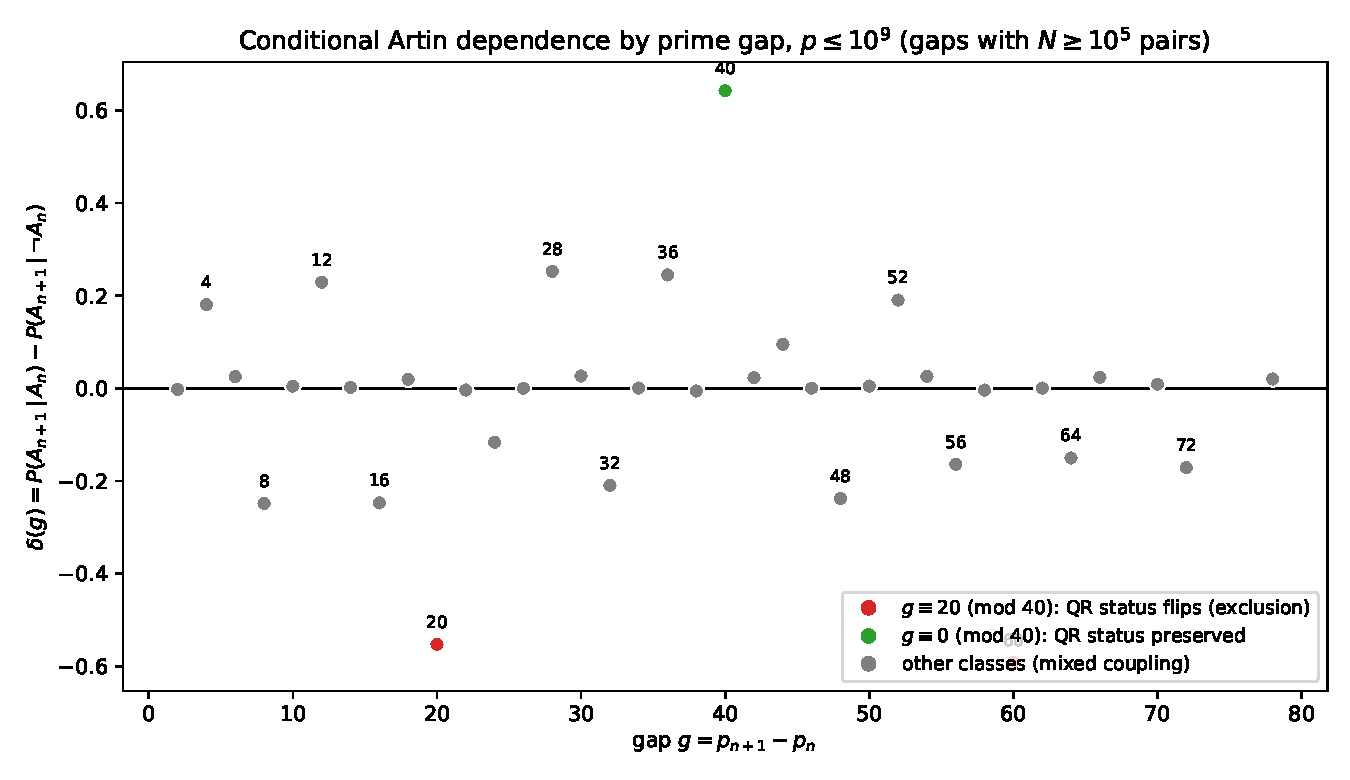
\includegraphics[width=0.95\textwidth]{fig_gap_delta.pdf}
	\caption{$\delta(g)$ for all gaps with $N \ge 10^5$ pairs, $p \le 10^9$. Red:
		$g \equiv 20 \pmod{40}$ (Theorem~\ref{thm:exclusion} forces
		$P(A|A) = 0$). Green: $g \equiv 0 \pmod{40}$
		(Corollary~\ref{cor:coupling} preserves quadratic-residue status). Grey: other
		classes.}
	\label{fig:gaps}
\end{figure}

Three features stand out.

\emph{(i) The exclusion rows.} At $g = 20$ ($1{,}824{,}043$ pairs) and $g = 60$
($371{,}839$ pairs), $P(A \mid A)$ is exactly zero: among $2.2$ million
consecutive pairs, not one is doubly Artin. This is
Theorem~\ref{thm:exclusion} in action, and conversely the observation that
motivated its proof.

\emph{(ii) The $g = 40$ spike.} $P(A \mid A) = 0.899$, the largest conditional
probability in the table and $2.4$ times the unconditional density. Two forced
mechanisms combine. First, by Corollary~\ref{cor:coupling}, if $p_n$ is Artin
then $10$ is a non-residue for $p_{n+1}$ as well, a necessary condition for
the Artin property.
Second, $40 \equiv 1 \pmod 3$ forces the pair's mod-$3$
residues: $p_n \equiv 2 \pmod 3$ would give $3 \mid p_n + 40$, impossible; so
every $g = 40$ pair has $p_n \equiv 1$, $p_{n+1} \equiv 2 \pmod 3$ --- that is,
$3 \mid p_n - 1$ (suppressing $\Art_n$) and $3 \nmid p_{n+1} - 1$ (favouring
$\Art_{n+1}$). Conditioning on $\Art_n$ therefore selects pairs in which
$p_{n+1}$ enjoys both the non-residue status and the mod-$3$ advantage.
These conditions are consistent with the large observed value $0.899$ but do
not quantitatively derive it without an explicit density calculation.

\emph{(iii) Sign classes.} Several gaps that are divisible by $3$ but not
constrained mod~$40$, for instance $6$, $18$, $30$, $42$ and $54$, show a
small positive $\delta \approx +0.02$. A natural guess is that the pair
shares its mod-$3$ status, weakly coupling the largest single suppression
factor. This is a
selected family rather than a rule: other gaps divisible by $3$ and lying in
neither $0$ nor $20$ mod~$40$, such as $12$, $24$ and $36$, do not all
behave this way, and we have no statement covering every class. Some gaps with
adverse mod-$8$ and mod-$5$ shifts show strong negative $\delta$. We can
therefore offer only a qualitative reading of Table~\ref{tab:gaps} in terms of
how the shift by $g$ permutes the residues of $p$ modulo $8$, $5$ and $3$; we
do not derive the entries, and outside the exclusion classes nothing here is
forced.

\section{Residue conditioning}
\label{sec:decomposition}

To what extent does the association persist once the explicit residue channels
are held fixed? We treat what follows as an exploratory conditioning
diagnostic; it does not answer that question quantitatively. We condition on
the \emph{joint} residue class of
$(p_n, p_{n+1})$ to modulus $m$ and measure the residual within-cell
dependence. The statistic reported is the sum of per-cell Pearson $\chi^2$
values over all non-degenerate cells meeting a minimum count threshold,
together with the pair-weighted mean of per-cell~$\delta$. This is a
descriptive aggregate of per-cell associations; it is \emph{not} the standard
Cochran--Mantel--Haenszel statistic (which would be a single one-degree-of-freedom
test of a common association).

Conditioning on $m = 120 = \mathrm{lcm}(8,3,5)$ fixes the quadratic character
$\Lsym{10}{\cdot}$ of both primes (its conductor $40$ divides $120$) and the
mod-$3$ channel. Cells in which $10$ is a quadratic residue for $p_n$ or
$p_{n+1}$ are degenerate for the analysis (one margin of the $2\times2$ table
vanishes --- the Artin property is impossible); the informative population is
roughly a quarter of all pairs, those in doubly-non-residue cells. The
selected populations in Table~\ref{tab:decomp} are the thresholded subsets of
this population: $12{,}255{,}203$ pairs ($24.10\%$ of the census) at
modulus~$120$ and $12{,}086{,}765$ pairs ($23.77\%$) at modulus~$840$. The
unthresholded doubly-non-residue fraction need not be exactly $1/4$.

\begin{table}[ht]
	\centering
	\caption{Selected-cell residual association after conditioning on joint residues
		mod $m$.
		``$\delta_{\mathrm{res}}$'' is the pair-weighted mean within-cell $\delta$
		over non-degenerate cells meeting the count threshold;
		``cells'' is the number of such cells; ``pairs used'' is the total pairs
		in those cells. Cells with fewer than $5000$ ($m = 120$) or $2000$ ($m = 840$)
		pairs are excluded.}
	\label{tab:decomp}
	\begin{tabular}{lrrrr}
		\toprule
		Conditioning           & cells & pairs used     & $\sum \chi^2$ (df) & $\delta_{\mathrm{res}}$ \\
		\midrule
		none (global)          & 1     & 50{,}847{,}530 & 10{,}167 \ (1)     & $-0.014140$             \\
		mod 120 joint residues & 145   & 12{,}255{,}203 & 789.2 \ (145)      & $-0.001055$             \\
		mod 840 joint residues & 633   & 12{,}086{,}765 & 719.8 \ (633)      & $-0.000473$             \\
		\bottomrule
	\end{tabular}
\end{table}

\textbf{Interpretation and limitations.}
The three statistics in Table~\ref{tab:decomp} have successively smaller
absolute values: $-0.0141$ (global) then $-0.00106$ (mod~$120$, $145$~cells
covering $12.3$~million pairs) then $-0.00047$ (mod~$840$, $633$~cells
covering $12.1$~million pairs). We emphasise that these are three different
quantities computed on three different populations, not one quantity being
reduced; the comparison is an exploratory conditioning diagnostic, not a
decomposition. Note also that a signed mean can be small because sizable
positive and negative within-cell associations cancel, so smallness in this
metric is not by itself evidence that dependence has gone. The summed per-cell
$\chi^2$ at mod~$840$ is $719.8$ on $633$ nominal degrees of freedom
($\chi^2/\mathrm{df} = 1.14$); we do not read $\chi^2/\mathrm{df} \approx 1$
as the disappearance of dependence, since no reference distribution has been
established for this serially structured, selected collection.
Two further observations: (i) the three values decrease in magnitude in the
order stated ($-0.0141$, $-0.00106$, $-0.00047$); (ii) a
split-sample check (pairs with $p < 5 \times 10^8$ versus
$p \ge 5 \times 10^8$, conditioning mod $120$) gives residuals
$-0.00096$ and $-0.00094$ --- stable across the range.

Several caveats apply. The global $\delta$ over $50.8$ million pairs and the
selected-cell $\delta_{\mathrm{res}}$ over $12.1$~million selected informative
pairs are \emph{different estimands on different populations}; arithmetic
comparison of their magnitudes is descriptive but does not constitute a proper
decomposition. A marginal risk difference is not, in general, the pair-weighted
mean of stratum risk differences without a between-group term and specified
weights. The per-cell Pearson calibration assumes independent observations
within each cell, which is not established for this serially structured
deterministic census. The paper does not specify a numerical model for the
omitted channels against which ``compatible'' could be formally tested. Those
omitted channels are not only the divisibility channels at $q \ge 11$:
fixing $p$ modulo $840$ determines whether $3$, $5$ and $7$ divide $p - 1$,
but not whether $10^{(p-1)/q} \equiv 1 \pmod p$ when one of them does, so
cubic and higher power-residue obstructions at these same small primes are
also unmodelled. The mod-$3$ channel here is the divisibility channel, not the
full cubic-residue condition.

Joint-residue conditioning yields a smaller selected-cell signed
residual association than the global figure. The remaining association is small in that metric but is
not established to vanish. These results are consistent with a substantial role
for arithmetic residue structure; they do not constitute a complete
decomposition or an independent quantitative verification of the
Hardy--Littlewood-based explanation of the consecutive-prime bias.

\section{The intermediate link: repulsion of \texorpdfstring{$\omega(p-1)$}{omega(p-1)}}
\label{sec:omega}

The chain from residue bias to Artin status passes through the factorisation
of $p - 1$. Its first summary statistic is
$\omega(p-1)$, the number of distinct prime factors, which has normal order
$\log\log p$ over shifted primes $p - 1$ --- a classical result of
Erd\H{o}s~\cite{Erdos1935}. (We invoke the normal order only; we do not use a
mean-value asymptotic, which would need separate tail control.) If consecutive primes repel modulo every small
$q$, then $q \mid p_n - 1$ makes $q \mid p_{n+1} - 1$ \emph{less} likely than
average, and summing over $q$ one predicts a negative correlation between
$\omega(p_n - 1)$ and $\omega(p_{n+1} - 1)$.

The data confirm this with a value that is, to our knowledge, unreported:
\[
	r\bigl(\omega(p_n - 1),\, \omega(p_{n+1} - 1)\bigr) = -0.0410
	\qquad (50{,}847{,}530 \text{ pairs}, \; p \le 10^9).
\]
The factorisations of $p - 1$ for consecutive primes are therefore not
independent. We stress that this measurement establishes dependence, not its
cause. The heuristic above accounts only for the same-$q$ terms: writing
$I_q(p) = \mathbf{1}_{q \mid p-1}$,
\[
  \operatorname{Cov}\bigl(\omega(p_n-1), \omega(p_{n+1}-1)\bigr)
  = \sum_q \operatorname{Cov}\bigl(I_q(p_n), I_q(p_{n+1})\bigr)
  + \sum_{q \ne r} \operatorname{Cov}\bigl(I_q(p_n), I_r(p_{n+1})\bigr),
\]
and the cross terms $q \ne r$ are neither estimated nor signed here. Summing
fixed-modulus predictions over all $q$ up to a growing cutoff would in any case
require uniformity and tail control that we do not supply. Nor is $\omega$ a
sufficient statistic for Artin status: which primes divide $p-1$, and whether
$10$ is a $q$th power residue, both matter. The observed repulsion is
consistent with the same residue-class repulsion that governs the primes, but
we do not establish that it has the same cause. The Pearson coefficient is
reported as a descriptive nominal value.

\section{Open questions}
\label{sec:questions}

The Hardy--Littlewood-based framework of~\cite{LOS2016} makes the residue
transition frequencies of consecutive primes quantitatively predictable, and
every channel in our conditioning is built from such frequencies. This
motivates the following open questions.

\begin{conjecture}[Persistence]
	\label{conj:persist}
	For primes up to $x$, the consecutive-pair Artin correlation
	$\delta(x) = P(\Art_{n+1} \mid \Art_n) - P(\Art_{n+1} \mid \lnot\Art_n)$
	is negative for all sufficiently large $x$.
\end{conjecture}

We have measured $\delta$ at four decade-spaced cutoffs:
\[
  \delta(10^8) = -0.013360, \quad
  \delta(10^9) = -0.014140, \quad
  \delta(10^{10}) = -0.014723, \quad
  \delta(10^{11}) = -0.014998 ,
\]
the last two from an independent recomputation described in
Section~\ref{sec:data} (over $455{,}052{,}508$ and $4{,}118{,}054{,}810$
primes respectively). At these four cutoffs the magnitude of $\delta$
increases, and the increments $-0.000780$, $-0.000583$, $-0.000275$ decrease.
No turnover is observed over the measured range.

We draw no asymptotic conclusion from this. Four nested cumulative cutoffs are
not four independent observations, and they determine neither an eventual sign
nor a limit nor a decay rate. Two specific negative remarks are all that the
values support: the ratio of successive increments is not constant ($0.75$
then $0.47$), so a geometric increment model does not describe them ---
extrapolating geometrically from the first three values predicts
$\delta(10^{11}) \approx -0.01516$ against a measured $-0.014998$, a
discrepancy of $1.6 \times 10^{-4}$ --- and $\delta(x)\log x$ is not constant
($-0.246, -0.293, -0.339, -0.380$), so a bare $c/\log x$ law does not describe
them either.

It is worth recording explicitly that monotone strengthening with decelerating
increments does \emph{not} constrain the eventual rate, and in particular does
not exclude decay to zero. Writing $t = \log_{10} x$, the function
\[
  f(t) = -\frac{0.248463}{t} - \frac{1.495239}{t^2}
         + \frac{41.285554}{t^3} - \frac{162.098640}{t^4}
\]
reproduces all four measured values at $t = 8, 9, 10, 11$, is negative for all
$t \ge 8$, strengthens across the measured range, and yet satisfies
$f(t) \sim -0.248463/t$, so that $f \to 0$; its turning point lies at
$t \approx 11.56$, just beyond the last cutoff. This is an interpolation
constructed to make the point, not a proposed model, and we attach no
significance to its coefficients. It shows only that our data are equally
compatible with eventual decay to zero and with persistence of a nonzero
correlation, and that the question is not settled by extending the census a
decade or two further.

We also note that the conjecture as stated --- that $\delta$ is eventually
negative --- is compatible with $\delta(x) \to 0$; eventual negativity and
decay to zero are not competing alternatives. A separate
reason for caution against assuming a nonzero limit arises in a restricted setting.
Consider a \emph{separable} fixed-modulus channel model: write $R, S$ for the
residue classes of $(p_n, p_{n+1})$ modulo a fixed~$M$, and suppose the
modelled indicators satisfy $\E[X \mid R,S] = \alpha(R)$,
$\E[Y \mid R,S] = \beta(S)$ and $\operatorname{Cov}(X, Y \mid R,S) = 0$, so
that the only modelled dependence between the two endpoints runs through the
joint law of $(R,S)$. If that joint law tends to the product of its
marginals, as the leading term of the Lemke Oliver--Soundararajan prediction
gives for fixed~$M$~\cite{LOS2016}, then
$\E[XY] - \E[X]\,\E[Y] \to 0$, and hence the modelled $\delta \to 0$ whenever
the limiting source marginal is nondegenerate. Non-uniform singular-series
weights across gap classes do not by themselves defeat this conclusion: the
gaps grow with~$x$, and it is the surviving total covariance, rather than the
non-uniformity of the weights, that would have to be estimated.

The separability hypothesis is essential and is not automatic. Conditioning
on the joint pair $(R,S)$ alone does not force independence: taking $R,S$
independent and uniform on the sixteen reduced classes modulo~$40$ and setting
$X = Y = Q(R)Q(S)$, where $Q$ indicates the eight classes on which the
relevant quadratic symbol is~$-1$, gives perfectly equidistributed residue
pairs together with $\E[X] = \E[Y] = \E[XY] = \tfrac14$ and
$\operatorname{Cov}(X,Y) = \tfrac{3}{16}$. So the observation above constrains
separable finite-modulus models, not every model built on a fixed modulus.
Extending a finite-obstruction approach to a statement about the limit would
in addition require joint-distribution information at each finite channel
together with a uniform bound on the omitted higher-power-residue
obstructions; the quadratic channel visible here is only the first of these.
The question of the limiting behaviour is unresolved; finite-range
measurements cannot distinguish the two alternatives.

\textbf{Research question (residue completeness).}
Does there exist, for every $\varepsilon > 0$, a modulus~$M$ such that
conditioning on the joint residues of $(p_n, p_{n+1})$ modulo~$M$ reduces
some appropriate within-cell dependence measure below~$\varepsilon$ in
absolute value? This is stated as a question rather than a conjecture because
a precise formulation requires specifying the order of limits (over~$x$
and~$M$), the treatment of sparse and degenerate cells, the dependence
criterion (e.g.\ a covariance decomposition rather than a signed cell mean),
and the range of~$x$ over which the bound is asserted. We do not know a
formulation that avoids these ambiguities.

We remark that a sufficiently uniform Hardy--Littlewood prime $k$-tuple
framework, together with a justified treatment of the no-intermediate-prime
restriction, would be the natural setting in which to predict the joint
distribution of $(p_n \bmod M, p_{n+1} \bmod M, g)$ via singular series. The
pair conjecture alone does not suffice, and the restriction is not an optional
refinement: consecutiveness is part of the event, and its indicator
\[
  \mathbf{1}_{p \text{ prime}} \, \mathbf{1}_{p+g \text{ prime}}
  \prod_{1 \le h < g} \bigl(1 - \mathbf{1}_{p+h \text{ prime}}\bigr)
\]
expands into higher-tuple correlations that two-point counts do not determine.
This is why~\cite{LOS2016} proceeds from a $k$-tuple heuristic rather than from
the pair conjecture. Whether such predictions carry the Chebotarev and
power-residue information needed for Artin status is a further question again,
and requires analysis we do not attempt here.

\begin{conjecture}[$\omega$ repulsion]
	\label{conj:omega}
	$r\bigl(\omega(p_n-1), \omega(p_{n+1}-1)\bigr)$ is negative for all large $x$
	and tends to $0$ as $x \to \infty$.
\end{conjecture}

The single reported value does not establish eventual sign or limit. We state
this as a conjecture consistent with the data.

\section{Discussion}
\label{sec:discussion}

\subsection*{What is new here}
The individual ingredients are classical: quadratic reciprocity, the
quadratic-residue obstruction to primitive roots, and the consecutive-prime bias
of~\cite{LOS2016}. The contributions of this paper are (i) the observation
that these combine into a deterministic exclusion law for prime pairs at gaps
$\equiv 20 \pmod{40}$ (Theorem~\ref{thm:exclusion}) --- elementary, but we have
not found it stated elsewhere; (ii) a measurement of the
consecutive-prime Artin correlation, its gap profile, and the $\omega$
repulsion; and (iii) evidence that arithmetic residue structure is substantially
connected to the measured dependence. The theorem is an immediate
application of standard quadratic reciprocity; its simplicity is a feature,
not a limitation.

\subsection*{Relation to runs of Artin primes}
Pollack~\cite{Pollack2014} proved (under GRH) that for every nonsquare
$g \neq -1$ and every~$m$, there are infinitely many runs of~$m$ consecutive
primes each having $g$ as a primitive root. Baker and
Pollack~\cite{BakerPollack2016} proved unconditionally that if~$Q$ contains
at least $\exp(Cm)$ multiplicatively independent primes, then infinitely many
runs of~$m$ consecutive primes each have some element of~$Q$ as a primitive
root, with the primes lying in a bounded-length interval.
Our results add an arithmetic constraint to the base-specific version:
for base~$10$, no run of all-Artin consecutive primes can cross a gap
$\equiv 20 \pmod{40}$. We have not inferred longer-run frequencies from the
pair statistic.

\subsection*{Future work}
Three extensions suggest themselves. (1) Other bases: the same pipeline with
$a = 2, 3, 5, 6, 7$ would test the conductor prediction of the Remark after
Corollary~\ref{cor:coupling} (e.g.\ conductor $8$ for $a = 2$, so exclusion
classes mod $8$; conductor $24$ for $a = 6$). (2) Scale: extending to
$10^{12}$ would help distinguish decay from persistence. (3) Theory: a
derivation of $\delta(g)$ from the singular series of~\cite{HardyLittlewood1923}
combined with the density computations of Hooley's method, at least for the
dominant channels, appears feasible and would replace our empirical
conditioning with a formula.

\section*{Acknowledgements}
The author thanks the developers of the open-source tools used in this work
(GMP, Python, NumPy, SymPy, Matplotlib).

\subsection*{Use of AI assistance}
A large-language-model AI assistant was used in code development,
literature-search assistance, drafting and editing, and initial formulation
of the elementary proof of Theorem~\ref{thm:exclusion}. The current revision
also used AI assistance for copy-editing and error correction. Numerical
outputs were produced by executing deterministic programs, not synthesised as
data by a language model. The author takes responsibility for the manuscript.

\section*{Declaration of interest}
No potential conflict of interest was reported by the author.

\section*{Funding}
This research received no specific grant from any funding agency in the
public, commercial, or not-for-profit sectors.

\section*{Data availability}
All code required to reproduce every number in this paper is supplied in the
accompanying reproduction package (C segmented sieve, Python analysis scripts,
figure script, and raw output logs). The code, manuscript, results and Lean
development are at
\url{https://github.com/jpbald93/consecutive-primitive-roots}, a repository
dedicated to this paper; the full per-prime CSV is not included there. That
package contains both implementations of the census described above, so a
reader can repeat the independent check as well as the original computation.
The sieve limit is configurable via a command-line argument, and the scripts
accept their input and output paths as arguments, defaulting to
repository-relative locations.
The per-prime dataset itself ($1.8$~GB CSV covering all $50{,}847{,}531$
primes from $7$ to $999{,}999{,}937$: gap, $\omega(p-1)$, Artin indicator,
and small residues for each prime) is not deposited because of its size, but
it is exactly and deterministically reproducible from the included C source on
a single machine; it is also available from the author on request.

\begin{thebibliography}{99}

	\bibitem{Artin1965}
	E.~Artin,
	\emph{The Collected Papers of Emil Artin} (S.~Lang and J.~T. Tate, eds.),
	Addison--Wesley, Reading, MA, 1965.

	\bibitem{BakerPollack2016}
	R.~C. Baker and P.~Pollack,
	\emph{Bounded gaps between primes with a given primitive root, II},
	Forum Math. \textbf{28} (2016), no.~4, 675--687.

	\bibitem{ConwayGuy1996}
	J.~H. Conway and R.~K. Guy,
	\emph{The Book of Numbers},
	Springer-Verlag, New York, 1996.

	\bibitem{Erdos1935}
	P.~Erd\H{o}s,
	\emph{On the normal number of prime factors of $p-1$ and some related problems
		concerning Euler's $\varphi$-function},
	Quart. J. Math. Oxford Ser. \textbf{6} (1935), 205--213.

	\bibitem{FanPollack2025}
	K.~(S.)~Fan and P.~Pollack,
	\emph{Counting primes with a given primitive root, uniformly},
	Mathematika \textbf{71} (2025), no.~4, Paper No.~e70055.

	\bibitem{GarciaKahoroLuca2019}
	S.~R. Garcia, E.~Kahoro, and F.~Luca,
	\emph{Primitive root bias for twin primes},
	Exp. Math. \textbf{28} (2019), no.~2, 151--160.

	\bibitem{GarciaLucaShiUdell2020}
	S.~R. Garcia, F.~Luca, K.~Shi, and G.~Udell,
	\emph{Primitive root bias for twin primes II: Schinzel-type theorems for
		totient quotients and the sum-of-divisors function},
	J. Number Theory \textbf{208} (2020), 400--417.

	\bibitem{GuptaMurty1984}
	R.~Gupta and M.~R. Murty,
	\emph{A remark on Artin's conjecture},
	Invent. Math. \textbf{78} (1984), no.~1, 127--130.

	\bibitem{HardyLittlewood1923}
	G.~H. Hardy and J.~E. Littlewood,
	\emph{Some problems of `Partitio numerorum'; III: On the expression of a
		number as a sum of primes},
	Acta Math. \textbf{44} (1923), 1--70.

	\bibitem{HeathBrown1986}
	D.~R. Heath-Brown,
	\emph{Artin's conjecture for primitive roots},
	Quart. J. Math. Oxford Ser. (2) \textbf{37} (1986), no.~145, 27--38.

	\bibitem{Hooley1967}
	C.~Hooley,
	\emph{On Artin's conjecture},
	J. Reine Angew. Math. \textbf{225} (1967), 209--220.

	\bibitem{KlurmanShparlinskiTeravainen2025}
	O.~Klurman, I.~E. Shparlinski, and J.~Ter\"av\"ainen,
	\emph{On Artin's conjecture on average and short character sums},
	Bull. Lond. Math. Soc. \textbf{57} (2025), no.~8, 2429--2443;
	\texttt{arXiv:2412.13355}.

	\bibitem{TinkovaWaxmanZindulka2023}
	M.~Tinkov\'a, E.~Waxman, and M.~Zindulka,
	\emph{Artin twin primes},
	J. Number Theory \textbf{247} (2023), 274--304;
	\texttt{arXiv:2010.15988}.

	\bibitem{LOS2016}
	R.~J. Lemke~Oliver and K.~Soundararajan,
	\emph{Unexpected biases in the distribution of consecutive primes},
	Proc. Natl. Acad. Sci. USA \textbf{113} (2016), no.~31, E4446--E4454.

	\bibitem{Moree2012}
	P.~Moree,
	\emph{Artin's primitive root conjecture --- a survey},
	Integers \textbf{12A} (2012), Article A13, 100~pp.

	\bibitem{PeruccaShparlinski2025}
	A.~Perucca and I.~E. Shparlinski,
	\emph{Uniform bounds for the density in Artin's conjecture on primitive roots},
	Bull. Lond. Math. Soc. \textbf{57} (2025), 978--991.

	\bibitem{Pollack2014}
	P.~Pollack,
	\emph{Bounded gaps between primes with a given primitive root},
	Algebra Number Theory \textbf{8} (2014), no.~7, 1769--1786.

\end{thebibliography}

\end{document}
